% =========================================================
%  AgentShield: IEEE-Style Technical Report
%  Deterministic Out-of-Band Security for Action-Taking AI Agents
% =========================================================
\documentclass[10pt,conference]{IEEEtran}

\usepackage[utf8]{inputenc}
\usepackage[T1]{fontenc}
\usepackage{amsmath}
\usepackage{amssymb}
\usepackage{graphicx}
\usepackage{hyperref}
\usepackage{url}
\usepackage{xcolor}
\usepackage{booktabs}
\usepackage{array}
\usepackage{tabularx}
\usepackage{listings}
\usepackage{microtype}
\usepackage{cite}
\usepackage{tikz}
\usetikzlibrary{shapes.geometric, arrows.meta, positioning, calc, fit, backgrounds}

% ---- TikZ style definitions ----
\tikzset{
  box/.style={
    rectangle, rounded corners=3pt,
    minimum width=2.5cm, minimum height=0.65cm,
    text centered, align=center,
    draw=black, font=\scriptsize, fill=gray!10
  },
  trustedbox/.style={box, fill=green!12, draw=green!60!black},
  untrustedbox/.style={box, fill=red!10, draw=red!60!black},
  humanbox/.style={box, fill=blue!10, draw=blue!60!black},
  storebox/.style={
    rectangle, rounded corners=2pt, minimum width=2.6cm, minimum height=0.6cm,
    text centered, align=center,
    draw=black!70, font=\scriptsize\itshape, fill=yellow!15, double
  },
  pipebox/.style={
    rectangle, rounded corners=2pt,
    minimum width=4.0cm, minimum height=0.50cm,
    text centered, align=center,
    draw=black, font=\scriptsize, fill=gray!10
  },
  passbox/.style={pipebox, draw=green!50!black, fill=green!10},
  denybox/.style={
    rectangle, rounded corners=2pt,
    minimum width=2.0cm, minimum height=0.45cm,
    text centered, align=center,
    draw=red!70!black, font=\scriptsize, fill=red!12
  },
  arrow/.style={-{Stealth[length=4pt]}, thick},
  dasharrow/.style={-{Stealth[length=4pt]}, thick, dashed},
  lbl/.style={font=\tiny, midway}
}

\lstset{
  basicstyle=\ttfamily\scriptsize,
  breaklines=true,
  frame=single,
  backgroundcolor=\color{gray!8}
}

\hypersetup{
  colorlinks=true,
  linkcolor=blue!60!black,
  citecolor=green!50!black,
  urlcolor=blue!70!black
}

% =========================================================
\begin{document}

\title{AgentShield: Deterministic Out-of-Band Enforcement\\
for Action-Taking AI Agents Against Prompt Injection}

\author{%
  \IEEEauthorblockN{Tejinderpal Singh, Rajput Yuvraj, and Ramswarup Swami}
  \IEEEauthorblockA{%
    \textit{Department of Computer Science and Engineering}\\
    \textit{Indian Institute of Information Technology Vadodara}\\
    Gandhinagar, Gujarat, India
  }
}

\maketitle

% =========================================================
\begin{abstract}
Large language model (LLM) agents that can invoke external tools---sending
emails, querying databases, writing files---are increasingly deployed in
production environments. These agents introduce a new class of vulnerability:
\emph{indirect prompt injection}, where adversarial content embedded in data
the agent reads (web pages, email bodies, document attachments) redirects the
agent to perform unauthorized actions. Published in-band defenses---system
prompt instructions, injection classifiers, input delimiters---have been
bypassed by adaptive attackers in prior evaluations. AgentShield addresses
this by placing all enforcement \emph{outside} the model, at the tool-call
boundary, implemented as a deterministic reference monitor. The system combines
six interlocking mechanisms: Cedar-policy-based least-privilege authorization,
information-flow integrity labeling derived from Biba and Bell--LaPadula models,
cryptographic human-approval receipts bound to exact argument digests, a
tamper-evident hash-chained and Merkle-anchored audit ledger, bounded-latency
session revocation, and a dual-LLM quarantine that prevents untrusted bytes from
reaching the privileged planner. An 8-stage fail-closed decision pipeline enforces
these properties in a fixed, non-bypassable order. The evaluation framework
integrates with AgentDojo to measure benign utility, utility under attack, and
targeted attack success rate, together with a defense-aware adaptive attack suite
and a per-pillar ablation study.
\end{abstract}

\begin{IEEEkeywords}
prompt injection, AI agent security, reference monitor, information-flow
control, least privilege, human-in-the-loop, audit logging,
capability-based security
\end{IEEEkeywords}

% =========================================================
\section{Introduction}

The deployment of autonomous AI agents---systems in which an LLM iteratively
plans and executes tool calls to complete multi-step tasks---has grown rapidly
over 2024--2026. Tool-enabled agents can read and send email, query databases,
modify files, post to external services, and orchestrate sub-agents. This
expanded capability fundamentally changes the security picture: an agent is no
longer a chatbot that produces text; it is a software principal capable of
real-world side effects.

\subsection{The Prompt Injection Threat}
Indirect prompt injection was first analyzed systematically by Greshake et al.\
\cite{greshake2023not}. The core observation is simple: if an agent reads
untrusted content as part of its task---a web page, an email it was asked to
summarize, a spreadsheet row---any adversary who can influence that content can
embed instructions that the agent may obey as if they came from the legitimate
user. Unlike direct injection, which requires access to the conversation,
indirect injection requires only the ability to place text where the agent will
read it.

The practical severity became clear with the rapid adoption of tool-calling
LLMs. An injected instruction in a webpage might direct an agent to forward
the user's inbox to an attacker, approve a malicious transaction, or exfiltrate
credentials---all without any direct access to the model, its API keys, or
the operator's infrastructure.

\subsection{Why In-Band Defenses Fail}
The natural response---adding defensive system prompts, instruction markers, or
injection-detection classifiers---targets the model itself. Recent evaluation work shows that adaptive, defense-aware attackers can bypass
these controls at high rates \cite{zhan2024injecagent}. The fundamental problem
is structural:
a model cannot simultaneously be the entity a defense is trying to protect
\emph{and} the entity making the protection decision.

\subsection{Contribution}
AgentShield takes a different approach. All enforcement decisions are made by
deterministic, non-LLM code at the tool-call boundary. LLMs appear in exactly
two narrowly scoped, non-authoritative roles---initial policy synthesis and
untrusted-data parsing---and neither can grant itself privilege. Contributions:

\begin{enumerate}
  \item A reference-monitor architecture for MCP tool
        calls implemented as a fail-closed 8-stage decision pipeline.
  \item A \emph{dual-LLM quarantine} that prevents untrusted bytes from
        reaching the privileged planner.
  \item A \emph{lethal-trifecta invariant} converting a security best
        practice into a runtime-enforced constraint.
  \item \emph{Cryptographic approval receipts} bound to the exact argument
        digest and a single-use nonce.
  \item A \emph{tamper-evident ledger} with Merkle-tree checkpoints.
  \item An \emph{evaluation framework} with AgentDojo \cite{agentdojo2024},
        defense-aware adaptive attacks, and per-pillar ablation.
\end{enumerate}

% =========================================================
\section{Problem Statement}

\subsection{Attacker Model}
The attacker is any entity that can place content into a channel the agent
reads. We assume an adaptive, defense-aware attacker who knows the system is
built on an LLM and knows AgentShield is in place; can control at least one
untrusted source the agent reads; cannot modify the gateway's code, signing
keys, or configuration; and may execute patient multi-step attacks.

\subsection{Structural Limitation of In-Band Solutions}
Any in-band defense places the model in the dual role of attack target and
defense mechanism. Both the legitimate instruction and the injection arrive via
the same channel and are processed by the same token prediction mechanism.
Classifiers face an analogous problem: an attacker knowing the decision
boundary can craft payloads that evade it.

\subsection{Design Requirement}
Effective enforcement must be outside the model, at the tool-call boundary,
implemented as a \emph{reference monitor} \cite{anderson1972computer}: always
invoked, tamper-proof (no LLM in the enforcement path), and small enough to
verify.

% =========================================================
\section{Architecture Overview}

AgentShield is organized around seven functional subsystems
(Fig.~\ref{fig:architecture}), a web-based control-plane console, and a
benchmark evaluation harness. The decomposition separates the security
kernel from policy evaluation, gateway mediation, approvals, revocation,
observability, and evaluation; it is an architectural boundary rather than a
requirement on any particular deployment language or directory layout.

\begin{figure*}[t]
\centering
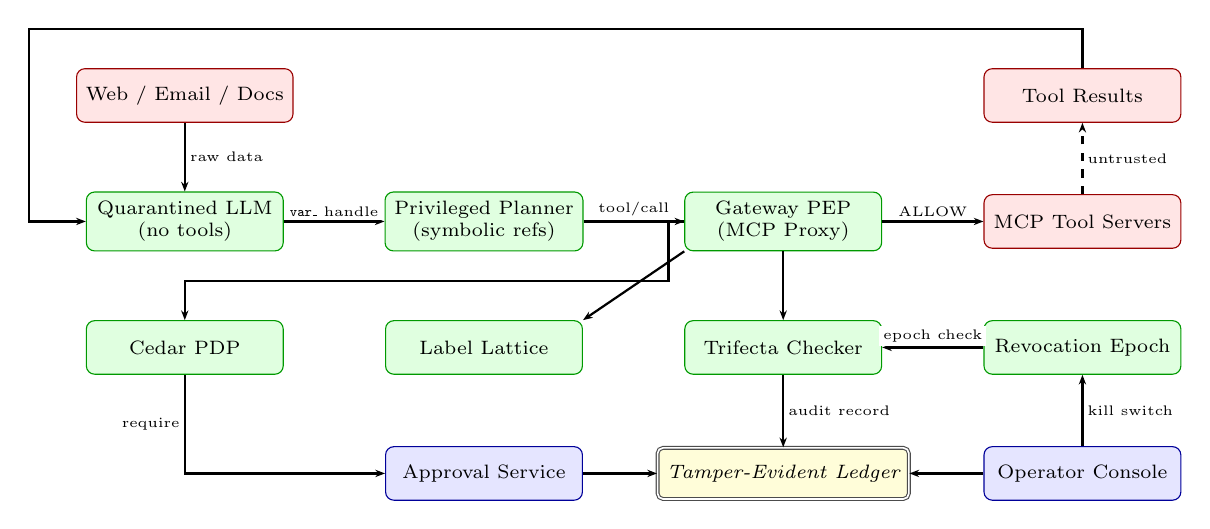
\begin{tikzpicture}[
  node distance=0.9cm and 1.1cm,
  tbox/.style={rectangle, rounded corners=3pt, minimum width=2.5cm,
               minimum height=0.68cm, text centered, align=center,
               draw=green!60!black, fill=green!12, font=\scriptsize},
  ubox/.style={rectangle, rounded corners=3pt, minimum width=2.5cm,
               minimum height=0.68cm, text centered, align=center,
               draw=red!60!black, fill=red!10, font=\scriptsize},
  hbox/.style={rectangle, rounded corners=3pt, minimum width=2.5cm,
               minimum height=0.68cm, text centered, align=center,
               draw=blue!60!black, fill=blue!10, font=\scriptsize},
  sbox/.style={rectangle, rounded corners=2pt, minimum width=2.5cm,
               minimum height=0.65cm, text centered, align=center,
               draw=black!70, fill=yellow!15, font=\scriptsize\itshape, double},
  arr/.style={-{Stealth[length=3.5pt]}, thick},
  darr/.style={-{Stealth[length=3.5pt]}, thick, dashed},
  lbl/.style={font=\tiny, fill=white, inner sep=1.5pt}
]

%% 4 Distinct Columns with Explicit Absolute Positioning
%% Col 1 (x=0)
\node[ubox] (web)  at (0, 3.6) {Web / Email / Docs};
\node[tbox] (qllm) at (0, 2.0) {Quarantined LLM\\(no tools)};
\node[tbox] (pdp)  at (0, 0.4) {Cedar PDP};

%% Col 2 (x=3.8)
\node[tbox] (pllm) at (3.8, 2.0) {Privileged Planner\\(symbolic refs)};
\node[tbox] (ifc)  at (3.8, 0.4) {Label Lattice};
\node[hbox] (apr)  at (3.8, -1.2) {Approval Service};

%% Col 3 (x=7.6)
\node[tbox] (pep)    at (7.6, 2.0) {Gateway PEP\\(MCP Proxy)};
\node[tbox] (tri)    at (7.6, 0.4) {Trifecta Checker};
\node[sbox] (ledger) at (7.6, -1.2) {Tamper-Evident Ledger};

%% Col 4 (x=11.4)
\node[ubox] (toolres) at (11.4, 3.6) {Tool Results};
\node[ubox] (tools)   at (11.4, 2.0) {MCP Tool Servers};
\node[tbox] (epoch)   at (11.4, 0.4) {Revocation Epoch};
\node[hbox] (con)     at (11.4, -1.2) {Operator Console};

%% Flows - Ingress & Planning
\draw[arr] (web) -- (qllm) node[midway, right, lbl] {raw data};
\draw[arr] (qllm) -- (pllm) node[midway, above, lbl] {\texttt{var\_} handle};
\draw[arr] (pllm) -- (pep) node[midway, above, lbl] {tool/call};
\draw[arr] (pep) -- (tools) node[midway, above, lbl] {ALLOW};
\draw[darr] (tools) -- (toolres) node[midway, right, lbl] {untrusted};
\draw[arr] (toolres.north) -- ++(0,0.5) -| ([xshift=-0.6cm]web.west) |- (qllm.west);

%% Reference Monitor Evaluations
\draw[arr] (pep.south) -- (tri.north);
\draw[arr] (pep.south west) -- (ifc.north east);
\draw[arr] (pep.west) -- ++(-0.2, 0) |- ([yshift=0.5cm]pdp.north) -- (pdp.north);
\draw[arr] (epoch) -- (tri) node[midway, above, lbl] {epoch check};

%% Approvals, Audit & Emergency Controls
\draw[arr] (pdp.south) |- (apr.west) node[near start, left, lbl] {require};
\draw[arr] (apr) -- (ledger);
\draw[arr] (tri) -- (ledger) node[midway, right, lbl] {audit record};
\draw[arr] (con) -- (ledger);
\draw[arr] (con) -- (epoch) node[midway, right, lbl] {kill switch};

\end{tikzpicture}
\caption{AgentShield system architecture.
\textcolor{green!60!black}{Green} = trusted deterministic enforcement;
\textcolor{red!60!black}{Red} = untrusted data sources;
\textcolor{blue!60!black}{Blue} = human-in-the-loop components;
\textit{Yellow} = tamper-evident audit store.}
\label{fig:architecture}
\end{figure*}

\subsection{Functional Decomposition}
\begin{itemize}
  \item \textbf{Security kernel}: Label lattice, provenance DAG, capability
        tokens, typed decisions, and trifecta tracking. This layer has no
        external I/O and contains the primitive security invariants.
  \item \textbf{Policy and confinement}: Cedar authorization, protocol-schema
        translation, and theorem-assisted subsumption checking for monotonic
        policy updates.
  \item \textbf{Gateway mediation}: The protocol proxy and Policy Enforcement
        Point that executes the fixed eight-stage pipeline.
  \item \textbf{Approval and revocation services}: Ed25519 receipt handling,
        consequence tiering, epoch counters, kill-switch operation, and
        blast-radius reporting.
  \item \textbf{Audit and observability}: Hash-chain and RFC~6962 Merkle
        logging, signed checkpoints, independent verification, and
        OpenTelemetry-compatible decision traces.
  \item \textbf{Agent integration}: Framework adapters, dual-LLM quarantine,
        and opaque-handle management at the boundary between untrusted data
        and the privileged planner.
  \item \textbf{Evaluation}: Standard benchmark integration, adaptive attack
        scenarios, local enforcement measurements, and per-pillar ablations.
\end{itemize}

% =========================================================
\section{The 8-Stage Decision Pipeline}

Every tool call passes through a fixed-order pipeline
(Fig.~\ref{fig:pipeline}). The pipeline is fail-closed: any exception,
timeout, parse error, or unresolved identity resolves to \texttt{DENY}.
No later stage can re-permit a denial issued by an earlier one.

\begin{figure}[t]
\centering
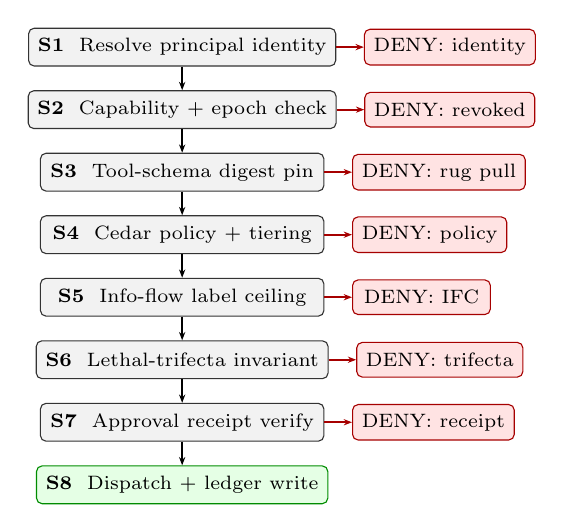
\begin{tikzpicture}[
  node distance=0.30cm,
  pbox/.style={rectangle, rounded corners=2pt,
               minimum width=3.6cm, minimum height=0.48cm,
               text centered, align=center,
               draw=black!80, fill=gray!10, font=\scriptsize},
  okbox/.style={pbox, draw=green!55!black, fill=green!10},
  dbox/.style={rectangle, rounded corners=2pt,
               minimum width=1.75cm, minimum height=0.44cm,
               text centered, align=center,
               draw=red!65!black, fill=red!11, font=\scriptsize},
  fa/.style={-{Stealth[length=3pt]}, thick},
  da/.style={-{Stealth[length=3pt]}, thick, red!65!black}
]
  \node[pbox] (s1) {\textbf{S1}\ \ Resolve principal identity};
  \node[pbox, below=of s1] (s2) {\textbf{S2}\ \ Capability + epoch check};
  \node[pbox, below=of s2] (s3) {\textbf{S3}\ \ Tool-schema digest pin};
  \node[pbox, below=of s3] (s4) {\textbf{S4}\ \ Cedar policy + tiering};
  \node[pbox, below=of s4] (s5) {\textbf{S5}\ \ Info-flow label ceiling};
  \node[pbox, below=of s5] (s6) {\textbf{S6}\ \ Lethal-trifecta invariant};
  \node[pbox, below=of s6] (s7) {\textbf{S7}\ \ Approval receipt verify};
  \node[okbox, below=of s7] (s8) {\textbf{S8}\ \ Dispatch + ledger write};

  \node[dbox, right=0.35cm of s1] (d1) {DENY: identity};
  \node[dbox, right=0.35cm of s2] (d2) {DENY: revoked};
  \node[dbox, right=0.35cm of s3] (d3) {DENY: rug pull};
  \node[dbox, right=0.35cm of s4] (d4) {DENY: policy};
  \node[dbox, right=0.35cm of s5] (d5) {DENY: IFC};
  \node[dbox, right=0.35cm of s6] (d6) {DENY: trifecta};
  \node[dbox, right=0.35cm of s7] (d7) {DENY: receipt};

  \foreach \a/\b in {s1/s2,s2/s3,s3/s4,s4/s5,s5/s6,s6/s7,s7/s8}
    \draw[fa] (\a) -- (\b);
  \foreach \a/\b in {s1/d1,s2/d2,s3/d3,s4/d4,s5/d5,s6/d6,s7/d7}
    \draw[da] (\a.east) -- (\b.west);
\end{tikzpicture}
\caption{The 8-stage fail-closed decision pipeline. The pipeline halts at the
first denial; all outcomes are written to the ledger unconditionally.}
\label{fig:pipeline}
\end{figure}

\subsection{Stage Descriptions}

\textbf{S1 -- Principal Identity.} Resolves an authenticated principal from
the request context. Unresolvable identity denies immediately.

\textbf{S2 -- Capability and Epoch.} Each call requires a capability
token encoding which tool is authorized, under what argument constraints
(caveats), for how long (TTL), and under which revocation epoch. A token
minted under an outdated epoch---the session was revoked---is rejected.

\textbf{S3 -- Tool-Schema Pinning.} At session start, the gateway records a
SHA-256 digest of each tool's advertised JSON schema and description. A
mismatch on subsequent calls is treated as a rug-pull supply-chain attack.

\textbf{S4 -- Cedar Policy + Approval Tiering.} The Cedar policy engine
evaluates typed arguments against the session's policy set (default-deny by
construction). A consequence-tiering layer then determines whether the call
additionally requires a human approval receipt.

\textbf{S5 -- Information-Flow Label Ceiling.} Every value carries a
\texttt{Label} (Biba integrity, Bell--LaPadula confidentiality). The session
accumulates a tightening label ceiling; a call violating it is denied with
a provenance explanation.

\textbf{S6 -- Lethal-Trifecta Invariant.} A session is denied from
acquiring the third ``leg'' when the other two are already held: (a)
untrusted input, (b) private data access, (c) external communication.

\textbf{S7 -- Approval Receipt.} When required, the gateway verifies an
Ed25519 receipt bound to the exact argument digest, resource version, a
single-use nonce, and an expiry.

\textbf{S8 -- Dispatch and Ledger.} On ALLOW, dispatches to the MCP
server. The outcome (\texttt{ok}, \texttt{denied}, or \texttt{uncertain}
for crashes) is written unconditionally to the append-only ledger.

% =========================================================
\section{Core Security Mechanisms}

\subsection{Information-Flow Label Lattice}

The label system implements Biba integrity \cite{biba1977integrity} combined
with Bell--LaPadula confidentiality \cite{bell1973secure}. The \texttt{Label}
type is an immutable pair of:
\begin{itemize}
  \item \texttt{Integrity} $\in$ \{UNTRUSTED, TENTATIVE, TRUSTED\}
  \item \texttt{Confidentiality} $\in$ \{PUBLIC, INTERNAL, PRIVATE, SECRET\}
\end{itemize}

When two values are combined, the join operation takes the more restrictive
of each dimension:
\begin{equation}
(i_1, c_1) \sqcup (i_2, c_2) = (\min(i_1, i_2), \;\max(c_1, c_2))
\end{equation}
This is associative, commutative, idempotent, and monotone, making it a valid
lattice join. Hypothesis property-based tests verify these four laws in the implementation;
a failing test would render the information-flow argument unsound.

A session's accumulated label can only tighten over time. Once a session
reads an untrusted source, its integrity ceiling cannot recover without
revocation.

\subsection{Dual-LLM Quarantine}

The dual-LLM pattern (Fig.~\ref{fig:dualllm}) prevents injected text from
reaching the privileged planner. All untrusted content is routed through a
\emph{quarantined} LLM that (a) holds zero tool bindings and (b) outputs
only structured data conforming to a Pydantic schema. The result is stored
behind an opaque \texttt{var\_} handle; the planner sees only the token
and never the raw bytes.

\begin{figure}[t]
\centering
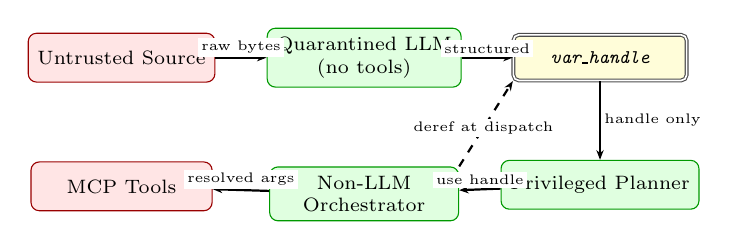
\begin{tikzpicture}[
  node distance=0.85cm and 0.55cm,
  ub/.style={rectangle, rounded corners=3pt, minimum width=2.3cm,
             minimum height=0.62cm, text centered, align=center,
             draw=red!60!black, fill=red!10, font=\scriptsize},
  qb/.style={rectangle, rounded corners=3pt, minimum width=2.4cm,
             minimum height=0.62cm, text centered, align=center,
             draw=green!60!black, fill=green!12, font=\scriptsize},
  sb/.style={rectangle, rounded corners=2pt, minimum width=2.2cm,
             minimum height=0.58cm, text centered, align=center,
             draw=black!70, fill=yellow!15, font=\scriptsize\itshape, double},
  ar/.style={-{Stealth[length=3.5pt]}, thick},
  dr/.style={-{Stealth[length=3.5pt]}, thick, dashed},
  lb/.style={font=\tiny, fill=white, inner sep=1.2pt}
]
  %% Top row
  \node[ub] (src)  {Untrusted Source};
  \node[qb, right=0.65cm of src]  (qllm) {Quarantined LLM\\(no tools)};
  \node[sb, right=0.65cm of qllm] (vh)   {\texttt{var\_handle}};

  %% Bottom row
  \node[ub, below=1.0cm of src]  (tools) {MCP Tools};
  \node[qb, below=1.0cm of qllm] (orch)  {Non-LLM\\Orchestrator};
  \node[qb, below=1.0cm of vh]   (pllm)  {Privileged Planner};

  %% Top flows
  \draw[ar] (src)  -- (qllm) node[midway, above, lb] {raw bytes};
  \draw[ar] (qllm) -- (vh)   node[midway, above, lb] {structured};
  \draw[ar] (vh)   -- (pllm) node[midway, right, lb] {handle only};

  %% Bottom flows
  \draw[ar] (pllm)  -- (orch)  node[midway, above, lb] {use handle};
  \draw[ar] (orch)  -- (tools) node[midway, above, lb] {resolved args};

  %% Diagonal dereference
  \draw[dr] (orch.north east) -- (vh.south west)
    node[pos=0.45, fill=white, inner sep=1.2pt, font=\tiny] {deref at dispatch};
\end{tikzpicture}
\caption{Dual-LLM quarantine. Raw untrusted bytes never reach the privileged
planner. The non-LLM orchestrator dereferences \texttt{var\_} handles only
at dispatch time; the planner only sees opaque tokens.}
\label{fig:dualllm}
\end{figure}

This design is derived from CaMeL \cite{camel2025}. Even if the quarantined
LLM is fully compromised, the entity dereferencing the handle is a non-LLM
orchestrator with no model to persuade.

\subsection{Monotonic Confinement}

The initial Cedar policy is synthesized by an LLM from the user's task
description. This is separate from the quarantined parser, and neither model
is authoritative. Every
subsequent policy update undergoes a \emph{subsumption check}: it must be a
provably narrower subset of the current policy to be auto-applied. Expansions
are held for human approval. The invariant: within a session, the action space
can only shrink without human involvement. A fully hijacked planner cannot
expand its own privilege.

The subsumption check uses Cedar's policy analyzer as the primary procedure,
with Z3 as a fallback for cases Cedar's analyzer does not cover.

\subsection{Tamper-Evident Audit Ledger}

The ledger is append-only enforced at the database grant level
(\texttt{INSERT}/\texttt{SELECT} only; \texttt{UPDATE}/\texttt{DELETE}
revoked). Each entry is chained:
\begin{equation}
h_n = H\!\bigl(\, h_{n-1} \;\|\; \mathrm{canonical}(e_n) \,\bigr)
\end{equation}
where \texttt{canonical} is RFC~8785 JSON canonicalization. Periodic Merkle
trees use RFC~6962 domain separation to prevent the CVE-2012-2459
duplicate-node collision. Signed checkpoints are published to an external
append-only anchor. A zero-dependency offline verifier allows third-party audit against a pinned
public key.

\subsection{Bounded-Latency Revocation}

The kill switch increments the session epoch, cancels all pending approvals,
and broadcasts an invalidation event so all gateway instances reject subsequent
calls immediately. Short capability TTLs ensure in-flight calls self-expire
quickly. Calls completed before propagation are recorded as \texttt{uncertain}
in a blast-radius report---the system is honest about what it cannot undo.

\subsection{Cryptographic Approval Receipts}

A single-use Ed25519 receipt binds: session, tool name, argument digest
$H(\text{args})$, resource version, nonce, and expiry. The argument digest
makes the receipt specific to exact bytes: any substitution of arguments
between approval and dispatch fails S7. The nonce is recorded in Redis on
first use and rejected on replay, closing both the replay attack and the
TOCTOU drift present in time-boxed approval schemes.

% =========================================================
\section{Implementation}

\subsection{Technology Stack}

\textbf{Policy engine.} Cedar \cite{cedar2023} is chosen over OPA/Rego
because it is authorization-specific, strongly typed, and default-deny by
construction. Its schema validator catches policy typos at load time. The Cedar
schema is auto-generated from the MCP server's \texttt{tools/list} response.

\textbf{Enforcement core.} Python~3.12, Pydantic~v2 for typed wire contracts,
the \texttt{cryptography} library for Ed25519, \texttt{rfc8785} for canonical
JSON. The core package has zero I/O dependencies.

\textbf{Gateway.} FastAPI with the MCP~v2 SDK (Streamable HTTP),
SQLAlchemy~2 async, asyncpg. Redis serves the approval queue and revocation
epoch store.

\textbf{Observability.} OpenTelemetry GenAI semantic conventions:
\texttt{gen\_ai.operation.name=execute\_tool}, correlated under an
\texttt{invoke\_agent} parent span. Policy decisions attach as span attributes.

\textbf{Quality gates.} Strict static typing, linting, dependency auditing,
and property-based tests verify label-lattice laws and
capability-attenuation monotonicity.

\subsection{Fail-Closed Implementation Pattern}

Every stage wraps its decision logic so any exception resolves to DENY:

\begin{lstlisting}[language=Python]
try:
    cedar_decision = self._pdp.authorize(
        session_id=request.session_id,
        tool_name=request.tool_name,
        arguments=request.arguments,
    )
except Exception as exc:
    return self._deny(
        request,
        Decision.deny(
            f"policy engine error, failing closed: {exc}",
            stage="cedar_policy",
        ),
    )
\end{lstlisting}

This is an architectural constraint: no code path in the enforcement layer can
turn an error into an ALLOW.

\subsection{Capability Token Design}

A capability token encodes tool name, argument caveats, the revocation epoch
at minting time, and an absolute TTL. Attenuation is append-only: a derived
capability can only add caveats, never remove them. Sub-agents in a
multi-agent chain cannot exceed their parent's privileges.

% =========================================================
\section{Evaluation Design}

\subsection{Standard Benchmark Metrics}

AgentShield integrates with AgentDojo \cite{agentdojo2024} through its
pipeline-extension interface. Three metrics are reported:

\begin{itemize}
  \item \textbf{Benign Utility (BU):} Fraction of legitimate tasks completed
    correctly with AgentShield enabled, without any injections. A default-deny
    system blocking legitimate work is a primary failure mode.
  \item \textbf{Utility Under Attack (UA):} Task completion rate when
    injection payloads are active.
  \item \textbf{Targeted ASR:} Fraction of injection tasks where the attacker's
    goal is achieved. Formally: $1 - \mathrm{mean}(\texttt{security\_results})$,
    read directly from AgentDojo's \texttt{SuiteResults}. Suites: Workspace,
    Slack, Travel, Banking.
\end{itemize}

\subsection{Defense-Aware Adaptive Attacks}

Most published defenses are evaluated on static attack payloads. AgentShield
includes three adaptive attacks targeting the two LLM roles rather than the
deterministic enforcement core:

\textbf{Policy Synthesizer Confusion.} Injects a fake authorized request to
widen the session policy. Structural defense: the confinement gate runs
subsumption checking; non-narrowing proposals are routed to
\texttt{REQUIRE\_APPROVAL} regardless of their claimed source.

\textbf{Approval Receipt Social Engineering.} Instructs the model to phrase
arguments to look benign to a human reviewer (homoglyphs in addresses, content
padded to hide attacker-controlled text). This targets reviewer attention, not
the cryptographic binding, and is included to measure a failure mode the
architecture does not claim to solve with cryptography alone.

\textbf{Quarantined Schema Injection.} Embeds fake JSON control sequences
hoping the quarantined LLM emits an embedded instruction. Structural defense:
the quarantined LLM returns only a handle; Pydantic rejects structurally
invalid output; the dereference entity is a non-LLM orchestrator.

\subsection{Per-Pillar Ablation}

To quantify the marginal contribution of each enforcement mechanism, the same
benchmark suite is run six times with one pillar neutralized per run
(Table~\ref{tab:ablation}). Neutralization reconfigures pluggable boundaries;
the fixed pipeline order is never patched.

\begin{table}[t]
\centering
\caption{Per-pillar ablation configurations}
\label{tab:ablation}
\begin{tabularx}{\columnwidth}{lX}
\toprule
\textbf{Configuration} & \textbf{Effect} \\
\midrule
\texttt{full} & All pillars active (baseline) \\
\texttt{no\_cedar\_policy} & Cedar replaced with permit-all policy \\
\texttt{no\_label\_lattice} & All ceilings widened to \texttt{Label.top()} \\
\texttt{no\_trifecta} & Trifecta legs cleared; S6 never denies \\
\texttt{no\_approval\_tiering} & No calls require approval \\
\texttt{unresponsive\_reviewer} & Tiering active; receipts never granted \\
\bottomrule
\end{tabularx}
\end{table}

The gap between \texttt{full} and any \texttt{no\_*} variant quantifies that
pillar's security contribution. The gap between \texttt{unresponsive\_reviewer}
and \texttt{full} measures the utility cost of approval fatigue.

\subsection{Local Enforcement Measurements}

Before running a live model-provider benchmark, we measured the reference
monitor in isolation using a reproducible local benchmark harness. Each
configuration used 1,000 samples. A sample consisted of one
benign egress call and two attack sequences: a policy-blocked exfiltration
attempt and an untrusted-read-then-egress attempt. Latency covers the
deterministic gateway evaluation and in-memory dispatch only; model inference,
network transport, and AgentDojo task execution are excluded.

\begin{table}[t]
\centering
\caption{Local enforcement measurements (1,000 samples/configuration)}
\label{tab:local-results}
\scriptsize
\begin{tabularx}{\columnwidth}{@{}Xrrrr@{}}
\toprule
\textbf{Configuration} & \textbf{BU} & \textbf{t-ASR} &
\textbf{Median} & \textbf{p95} \\
\midrule
\texttt{full} & 1.00 & 0.00 & 0.338 & 0.828 \\
\texttt{no\_cedar\_policy} & 1.00 & 0.00 & 0.300 & 0.676 \\
\texttt{no\_label\_lattice} & 1.00 & 0.50 & 0.316 & 0.685 \\
\texttt{no\_trifecta} & 1.00 & 0.00 & 0.322 & 0.971 \\
\texttt{unresponsive\_reviewer} & 0.00 & 0.00 & 0.564 & 1.710 \\
\bottomrule
\end{tabularx}
\end{table}

The full configuration blocked all 2,000 attack attempts while dispatching all
1,000 benign calls. Disabling the label lattice allowed one of the two attack
families through in every sample, yielding a 0.50 local t-ASR. An
unresponsive reviewer reduced benign utility to zero, quantifying the
approver-fatigue failure mode in this deliberately conservative configuration.
Because the local harness repeats fixed deterministic scenarios, the larger
sample is evidence of repeatability and stable overhead, not a confidence
interval over independent user tasks or model trajectories. These measurements
validate enforcement behavior and overhead, but they do not establish AgentDojo
utility or generalization; the live four-suite benchmark remains a separate
experiment requiring fixed model, seed, and provider documentation.

% =========================================================
\section{Trust Boundaries and Non-Goals}

\subsection{Trust Hierarchy}

Table~\ref{tab:trust} summarizes the four-level trust model. The critical
invariant: only the deterministic non-LLM layer may authorize a tool call.

\begin{table}[t]
\centering
\caption{Trust hierarchy in AgentShield}
\label{tab:trust}
\begin{tabularx}{\columnwidth}{lX}
\toprule
\textbf{Layer} & \textbf{Role} \\
\midrule
Untrusted & Web content, emails, docs, third-party tool results \\
Semi-trusted & Privileged LLM planner; denied raw untrusted bytes;
             cannot grant itself privilege \\
Trusted (non-LLM) & PDP, capability broker, ledger, approval and
                     revocation services; only these authorize calls \\
Human & Approver; trusted per-decision, not globally \\
\bottomrule
\end{tabularx}
\end{table}

\subsection{Explicit Non-Goals}

AgentShield does \emph{not}:
\begin{itemize}
  \item make the planner LLM immune to prompt injection at the model
        level---that boundary is assumed permanently permeable;
  \item treat injection classifiers as authoritative---they are
        defense-in-depth only, raising a call's approval tier;
  \item guarantee task utility---enforcement correctness is prioritized
        over task completion;
  \item protect against a compromised gateway host;
  \item undo external side effects; blast-radius reporting is honest about
        this limitation;
  \item address model misalignment on tasks the user genuinely authorized.
\end{itemize}

% =========================================================
\section{Related Work}

\textbf{Progent} \cite{progent2025} introduces symbolic privilege policies over
tool names and typed arguments with monotonic confinement via SMT-checked
policy updates. AgentShield extends this with information-flow labels,
cryptographic receipts, and a full gateway implementation.

\textbf{CaMeL} \cite{camel2025} (Google DeepMind/ETH Zurich) provides a
concrete dual-LLM quarantine. AgentShield's quarantine is directly inspired
by this design.

\textbf{FIDES} \cite{fides2025} (Microsoft) implements information-flow
control as agent middleware with label propagation. AgentShield's label
lattice follows the Biba+BLP model FIDES formalizes.

\textbf{AgentDojo} \cite{agentdojo2024} provides the benchmark harness.
Recent open-ended evaluation work extends this setting with dynamic injection
cases and measures both adaptive attack resilience and over-defense.

The primary differentiator of AgentShield is the combination of all mechanisms
in a single reference implementation, evaluated against attacks written with
knowledge of the defense's own source code.

% =========================================================
\begin{thebibliography}{12}

\bibitem{greshake2023not}
K.~Greshake, S.~Abdelnabi, S.~Mishra, C.~Endres, T.~Holz, and M.~Fritz,
``Not what you've signed up for: Compromising real-world LLM-integrated
applications with indirect prompt injection,''
in \emph{Proc.\ ACM AISec Workshop}, 2023.

\bibitem{agentdojo2024}
E.~Debenedetti et al.,
``AgentDojo: A dynamic environment to evaluate prompt injection attacks and
defenses for LLM agents,''
in \emph{Proc.\ NeurIPS 2024 Datasets and Benchmarks Track}, 2024.

\bibitem{zhan2024injecagent}
Q.~Zhan, F.~Luo, Z.~Li, Z.~Zhang, and C.~Yang,
``InjecAgent: Benchmarking indirect prompt injection attacks on
tool-integrated LLM agents,''
in \emph{Findings of ACL}, 2024.

\bibitem{progent2025}
L.~Chen, S.~Liu, X.~Wang, and Y.~Zhang,
``Progent: Securing AI agents with programmable privilege control,''
\emph{arXiv:2504.11703}, 2025.

\bibitem{camel2025}
E.~Debenedetti, J.~Ganz, K.~Gr\"{o}nvall, et al.,
``Defeating prompt injections by design,''
\emph{arXiv:2503.18813}, Google DeepMind / ETH Zurich, 2025.

\bibitem{fides2025}
M.~Russinovich, A.~Salem, and R.~Elidan,
``FIDES: Information-flow control for LLM agents,''
Microsoft Agent Framework Blog, 2025.

\bibitem{cedar2023}
Amazon Web Services,
``Cedar: A new policy language,'' 2023.
[Online]. Available: \url{https://www.cedarpolicy.com/}

\bibitem{biba1977integrity}
K.~J.~Biba,
``Integrity considerations for secure computer systems,''
MITRE Corporation, Tech.\ Rep.\ MTR-3153, 1977.

\bibitem{bell1973secure}
D.~E.~Bell and L.~J.~LaPadula,
``Secure computer systems: Mathematical foundations,''
MITRE Corporation, Tech.\ Rep.\ MTR-2547, 1973.

\bibitem{anderson1972computer}
J.~P.~Anderson,
``Computer security technology planning study,''
ESD-TR-73-51, USAF Electronic Systems Division, 1972.

\end{thebibliography}

\end{document}